\documentclass[a4paper,12pt]{article}

\usepackage[utf8]{inputenc}
\usepackage[T1]{fontenc}
\usepackage[frenchb]{babel} % If you write in French
%\usepackage[english]{babel} % If you write in English
\usepackage{listings}
\usepackage{a4wide}
\usepackage{graphicx}
\graphicspath{{images/}}
\usepackage{subfig}
\usepackage{tikz}
\usetikzlibrary{shapes,arrows}
\usepackage{pgfplots}
\pgfplotsset{compat=newest}
\pgfplotsset{plot coordinates/math parser=false}
\newlength\figureheight
\newlength\figurewidth
\pgfkeys{/pgf/number format/.cd,
set decimal separator={,\!},
1000 sep={\,},
}
\usepackage{ifthen}
\usepackage{ifpdf}
\ifpdf
\usepackage[pdftex]{hyperref}
\else
\usepackage{hyperref}
\fi
\usepackage{color}
\hypersetup{%
colorlinks=true,
linkcolor=black,
citecolor=black,
urlcolor=black}

\renewcommand{\baselinestretch}{1.05}
\usepackage{fancyhdr}
\pagestyle{fancy}
\fancyfoot{}
\fancyhead[L,RO]{\bfseries\thepage}
%\fancyhead[R]{\bfseries\nouppercase{\leftmark}}
\fancyhead[LO]{\bfseries\nouppercase{\leftmark}}
\setlength{\headheight}{15pt}
%\fancyfoot[C]{\textbf{page \thepage}} 

\let\headruleORIG\headrule
\renewcommand{\headrule}{\color{black} \headruleORIG}
\renewcommand{\headrulewidth}{1.0pt}
\usepackage{colortbl}
\arrayrulecolor{black}

\fancypagestyle{plain}{
  \fancyhead{}
  \fancyfoot[C]{\thepage}
  \renewcommand{\headrulewidth}{0pt}
}

\makeatletter
\def\@textbottom{\vskip \z@ \@plus 1pt}
\let\@texttop\relax
\makeatother

\makeatletter
\def\cleardoublepage{\clearpage\if@twoside \ifodd\c@page\else%
  \hbox{}%
  \thispagestyle{empty}%
  \newpage%
  \if@twocolumn\hbox{}\newpage\fi\fi\fi}
\makeatother

\usepackage{amsthm}
\usepackage{amssymb,amsmath,bbm}
\usepackage{array}
\usepackage{bm}
\usepackage{multirow}
\usepackage[footnote]{acronym}
\usepackage{pdfpages}
\usepackage{enumerate}
\usepackage{rotating}
\usepackage{titlesec}


\newcommand*{\SET}[1]  {\ensuremath{\mathbf{#1}}}
\newcommand*{\VEC}[1]  {\ensuremath{\boldsymbol{#1}}}
\newcommand*{\FAM}[1]  {\ensuremath{\boldsymbol{#1}}}
\newcommand*{\MAT}[1]  {\ensuremath{\boldsymbol{#1}}}
\newcommand*{\OP}[1]  {\ensuremath{\mathrm{#1}}}
\newcommand*{\NORM}[1]  {\ensuremath{\left\|#1\right\|}}
\newcommand*{\DPR}[2]  {\ensuremath{\left \langle #1,#2 \right \rangle}}
\newcommand*{\calbf}[1]  {\ensuremath{\boldsymbol{\mathcal{#1}}}}
\newcommand*{\shift}[1]  {\ensuremath{\boldsymbol{#1}}}

\newcommand{\eqdef}{\stackrel{\mathrm{def}}{=}}
\newcommand{\argmax}{\operatornamewithlimits{argmax}}
\newcommand{\argmin}{\operatornamewithlimits{argmin}}
\newcommand{\ud}{\, \mathrm{d}}
\newcommand{\vect}{\text{Vect}}
\newcommand{\sinc}{\ensuremath{\mathrm{sinc}}}
\newcommand{\esp}{\ensuremath{\mathbb{E}}}
\newcommand{\hilbert}{\ensuremath{\mathcal{H}}}
\newcommand{\fourier}{\ensuremath{\mathcal{F}}}
\newcommand{\sgn}{\text{sgn}}
\newcommand{\intTT}{\int_{-T}^{T}}
\newcommand{\intT}{\int_{-\frac{T}{2}}^{\frac{T}{2}}}
\newcommand{\intinf}{\int_{-\infty}^{+\infty}}
\newcommand{\Sh}{\ensuremath{\boldsymbol{S}}}
\newcommand{\C}{\SET{C}}
\newcommand{\R}{\SET{R}}
\newcommand{\Z}{\SET{Z}}
\newcommand{\N}{\SET{N}}
\newcommand{\K}{\SET{K}}
\newcommand{\reel}{\mathcal{R}}
\newcommand{\imag}{\mathcal{I}}
\newcommand{\cmnr}{c_{m,n}^\reel}
\newcommand{\cmni}{c_{m,n}^\imag}
\newcommand{\cnr}{c_{n}^\reel}
\newcommand{\cni}{c_{n}^\imag}
\newcommand{\tproto}{g}
\newcommand{\rproto}{\check{g}}
\newcommand{\LR}{\mathcal{L}_2(\SET{R})}
\newcommand{\LZ}{\ell_2(\SET{Z})}
\newcommand{\LZI}[1]{\ell_2(\SET{#1})}
\newcommand{\LZZ}{\ell_2(\SET{Z}^2)}
\newcommand{\diag}{\operatorname{diag}}
\newcommand{\noise}{z}
\newcommand{\Noise}{Z}
\newcommand{\filtnoise}{\zeta}
\newcommand{\tp}{g}
\newcommand{\rp}{\check{g}}
\newcommand{\TP}{G}
\newcommand{\RP}{\check{G}}
\newcommand{\dmin}{d_{\mathrm{min}}}
\newcommand{\Dmin}{D_{\mathrm{min}}}
\newcommand{\Image}{\ensuremath{\text{Im}}}
\newcommand{\Span}{\ensuremath{\text{Span}}}
\definecolor{deepblue}{rgb}{0,0,0.5}
\definecolor{deepred}{rgb}{0.6,0,0}
\definecolor{deepgreen}{rgb}{0,0.5,0}

\newcommand\cstyle{\lstset{
language=C,
%style=numbers,
basicstyle=\ttfamily\scriptsize,
%otherkeywords={self},{True},{False},             % Add keywords here
keywordstyle=\color{deepblue}\bfseries,
commentstyle=\color{deepred},
stringstyle=\color{deepgreen},
showstringspaces=false
frame=Trbl,
showstringspaces=false,
breaklines=true,
numbers=left
}}

\newcommand\cexternal[2][]{{
\cstyle
\lstinputlisting[#1]{#2}}}

\newtheoremstyle{break}
  {11pt}{11pt}%
  {\itshape}{}%
  {\bfseries}{}%
  {\newline}{}%
\theoremstyle{break}

%\theoremstyle{definition}

\parskip=5pt
%\sloppy

\newcommand\tab[1][1cm]{\hspace*{#1}} %tabulation

\titleformat{\paragraph}
{\normalfont\normalsize\bfseries}{\theparagraph}{1em}{}
\titlespacing*{\paragraph}
{0pt}{3.25ex plus 1ex minus .2ex}{1.5ex plus .2ex}

\setcounter{secnumdepth}{4}

\begin{document}

%%%%%%%%%%%%%%%%%%
%%% First page %%%
%%%%%%%%%%%%%%%%%%

\begin{titlepage}
\begin{center}

\begin{minipage}[c]{.46\linewidth}
     \begin{center}
             
\includegraphics[width=8cm]{TSP}
         \end{center}
   \end{minipage} \hfill
   \begin{minipage}[c]{.46\linewidth}
    \begin{center}
            
\includegraphics[width=8cm]{cassiopee}
        \end{center}
 \end{minipage}

%
\includegraphics[width=0.3\textwidth]{TSP}\\[0.2cm]
%
\includegraphics[width=0.3\textwidth]{cassiopee}\\[0.2cm]


{\large PRO4501 : Projet Cassiopée}\\[0.5cm]

{\large Hermès-LiDAR}\\[0.5cm]

% Title
\rule{\linewidth}{0.5mm} \\[0.4cm]
{ \huge \bfseries Rapport\\[0.4cm] }
\rule{\linewidth}{0.5mm} \\[1.5cm]

% Author and supervisor
\noindent
\begin{minipage}{0.4\textwidth}
  \begin{flushleft} \large
    \emph{Auteurs :}\\
    Mme Mélanie \textsc{COSMIDES}\\
    M. Ugurcan \textsc{EKREN}\\
    M. Florian \textsc{GRANTE}\\
  \end{flushleft}
\end{minipage}%
\begin{minipage}{0.4\textwidth}
  \begin{flushright} \large
    \emph{Encadrants :} \\
    M. Emmanuel \textsc{MONFRINI}\\
    M. Clément \textsc{BESNIER}\\
    M. Claude \textsc{VILLARD}\\
  \end{flushright}
\end{minipage}

\vfill

% Bottom of the page
{\large \today}

\end{center}
\end{titlepage}

%%%%%%%%%%%%%%%%%%%%%%%%%%%%%
%%% Non-significant pages %%%
%%%%%%%%%%%%%%%%%%%%%%%%%%%%%
\clearpage
\tableofcontents


%%%%%%%%%%%%%%%%%%%%%%%%%%%%%%%%%%%%%%%%%%%%
%%% Content of the report and references %%%
%%%%%%%%%%%%%%%%%%%%%%%%%%%%%%%%%%%%%%%%%%%%
\pagestyle{fancy}

\cleardoublepage

\section*{Remerciements}
\addcontentsline{toc}{section}{Remerciements}
\markboth{Remerciements}{Remerciements}

\tab Nous tenons à remercier Nexter de nous avoir fait confiance et nous avoir aidé financièrement dans ce projet. 

\tab Nous remercions également M. Claude Villard pour son aide à la mise en place de ce type de projet.

\tab Il nous tient également à coeur de remercier M.Monfrini et Clément Besnier qui nous accompagnés avec bienveillance lors de la réalisation technique de ce projet.

\tab Nous remercions également le Club INTech pour nous avoir prêté la plateforme robotique sur laquelle nous avons intégré notre projet.
\section*{Introduction}
\addcontentsline{toc}{section}{Introduction}
\markboth{Introduction}{Introduction}

\tab L'année derniere, le projer Hermès a été développé, visant la création d'une plateforme motorisée mobile permettant de guider des personnes dans le forum de Télécom SudParis. Cette année, l'objectif a été de lui ajouter un dispositif de détection afin de lui permettre de se repérer au sein de son environnement et de détecter d'éventuels obstacles. Pour cela, nous avons proposé l'utilisation d'un LiDAR (Light Detecion And Ranging), système permettant la récupération de nuages de points autour du système. Malheureusement, la plateforme Hermès n'étant pas en état de marche, nous nous sommes rabattu sur le robot du club INTech qui a participé avec notre système à la Coupe de France de Robotique afin de réaliser nos travaux qui seront détaillés dans ce dossier.

\tab Les dispositifs LiDAR sont très utilisés dans le monde de la robotique, notamment par Boston Dynamics ou encore Nexter. Ils permettent de cartographier le monde autour du robot afin d'interagir ou d'éviter des obstacles. Ils sont également omniprésents dans les projets de voiture autonome comme les récentes Tesla. Cependant, les données brutes d'un LiDAR sont très basiques, il faut alors tout un traitement en aval par des algorithmes qui formeront ce que nous pouvons appeler un véritable \textit{capteur logiciel}.

\tab Le problème posé est alors celui du traitement des données brutes d'un LiDAR dans l'objectif d'une détection d'obstacles et de localisation (un robot adverse par exemple dans ce cas précis) permettant à un algorithme de recherche de chemin de pouvoir oeuvrer. Cette recherche de chemin associé à notre LiDAR a fait l'oeuvre d'un second projet Cassiopée, Hermès - Pathfinding.

\section{Définition du cadre du projet}

\subsection{Analyse Benchmark}

\tab L'état de l'art de la détection d'obstacle est actuellement centrée sur les algorithmes dits de SLAM pour \textit{Simultaneous Localization and Mapping}\cite{slam-nexter}. Ces algorithmes sont extrêmement bien adaptés à l'utilisation d'un LiDAR sur un robot possédant d'autres capteurs de déplacements (les encodeurs rotatif incrémentaux sur les roues par exemple), car la fusion de ces capteurs avec les données du LiDAR permet de minimiser les imprécisions de mesure tout en gérant une carte dynamique de l'environnement. Cela permet de surcroît de positionner le robot lui-même dans son environnement. On corrige ainsi les décalages éventuels du robot et de ses encodeurs rotatifs. Plusieurs grandes phases sont discernables dans ce type d'algorithme :

\begin{enumerate}
    \item la récupération des données et le filtrage des données aberrantes,
    \item la recherche d'éléments reconnaissables (point de repères ou \textit{landmarks} dans la littérature),
    \item mise en lien des point de repères entre plusieurs mesures (association, détermination des mouvements),
    \item utilisation de ces point de repères, de la position supposée du robot par ses autres capteurs et de ses positions et cartographies précédentes pour construire la prochaine carte la plus probable.
\end{enumerate}

Actuellement, un très grand travail de recherche est effectué dans le domaine de l'automobile, entre autres, avec l'émergence des véhicules autonomes qui ont besoin d'acquérir énormément de données sur leur environnement. Des systèmes basés sur des LiDARs multicouches (fournissant des nuages de points en 3D et non en 2D comme le nôtre) permettent à ces véhicules de se repérer, éviter les obstacles et suivre la route sans danger.

\subsection{Prise en main du LiDAR}
\subsubsection{Installation}
\tab De nombreux documents et un logiciel de prise en main sont fournis par le constructeur, et les fournisseurs. Vous pourrez trouver entre autres la documentation officielle et un logiciel d’affichage de données en temps réel sur le lien suivant :\newline \href{https://www.robotshop.com/en/rplidar-a2-360-laser-scanner.html}{\textit{Lien vers le site robotshop.}}\footnote{https://www.robotshop.com/en/rplidar-a2-360-laser-scanner.html}

\begin{figure}[htp]
    \centering
    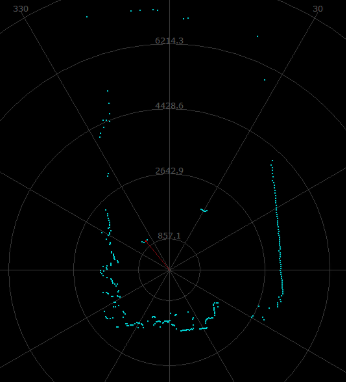
\includegraphics[width=6cm]{/Cadre/demo.PNG}
    \caption{Logiciel de démonstration du capteur fourni.}
\end{figure}

Pour nos premiers tests, nous avons utilisé une bibliothèque existante en Python permettant une prise en main rapide et sûre du lidar, avec des gestions de cas d’erreurs et de validité de données envoyées par le lidar.
\href{https://github.com/Roboticia/RPLidar}{\textit{Lien vers la bibliothèque.}}\footnote{https://github.com/Roboticia/RPLidar}


Nous avons également réalisé une plateforme de test fixe pour maîtriser le capteur avant de l’embarquer dans un robot:

\begin{figure}[htp]
    \centering
    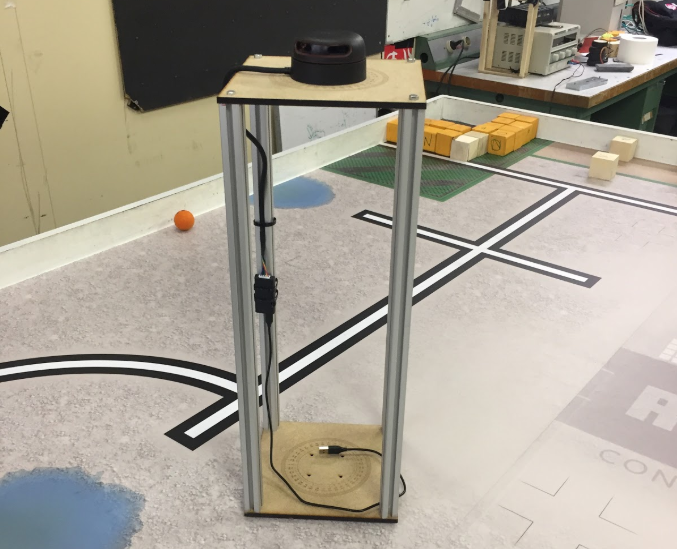
\includegraphics[width=6cm]{/Cadre/plateforme_test.PNG}
    \caption{Plateforme de test.}
\end{figure}

\subsubsection{Étude de la fiabilité du LiDAR}
\paragraph{Étude des valeurs aberrantes}
\tab Lors de nos premières phases de tests, nous avons pu observer la présence de valeurs aberrantes dans nos mesures, allant parfois jusqu'à plusieurs centimètres d'écart à la réalité. Mais la majorité des valeurs étant à quelques millimètres d'écarts, un filtrage simple doit permettre de retirer ces aberrations.
On remarque en outre une grande importance du choix de la vitesse en rotation, ces aberrations étant plus présentes à basses ou hautes vitesses, mais moins en vitesses moyennes, proches de celle par défaut à 10Hz.

\begin{figure}[htp]
    \centering
    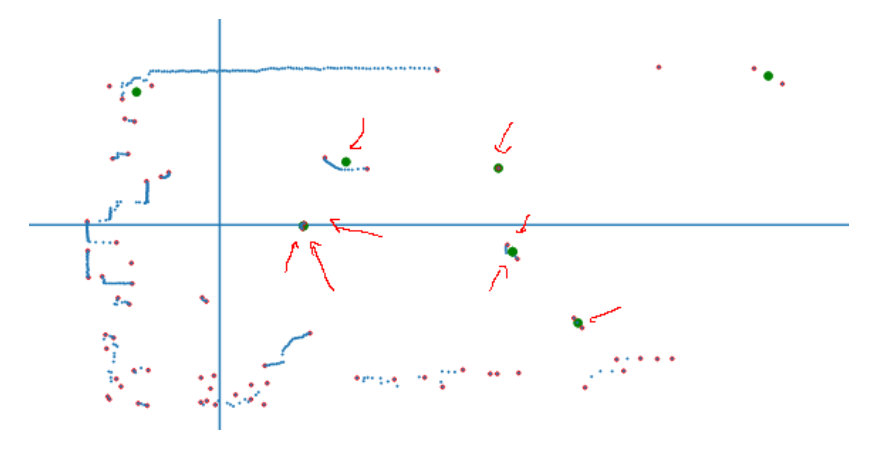
\includegraphics[width=6cm]{/Cadre/premier_test.PNG}
    \caption{Visuel du premier test réalisé avec le LiDAR.}
\end{figure}

\tab Par rapport à la documentation, on remarque également que la vitesse maximale réelle est 19Hz et pas 15Hz comme indiqué, mais nous resterons dans les standards (valeur conseillée étant de 60\% du PWM maximal, correspondant à une fréquence de mesure 10Hz) pour éviter d'user le composant et éviter d'endommager notre terminal, le port USB ne pouvant fournir qu'un courant limité dans le cas où l'alimentation du LiDAR se ferait uniquement par l'USB.

\paragraph{Choix d'une vitesse de rotation}

\tab Afin de déterminer une vitesse de rotation, nous avons procédé de la façon suivante :
Nous prenons des mesures sur 20 secondes. Pour un angle donné, on récupère les valeurs qui sont compris dans [Angle-0.5,Angle+0.49]. On trace alors un graphe pour chaque vitesse.

\tab On remarque alors qu'une vitesse basse donne des mesures plus dispersées et qu'un vitesse très élevée donne souvent un résultat proche de la réalité mais donne parfois un résultat biaisé.

\tab $ V \simeq 500$ (Ce qui correspond à un PWM à 48.8\%) semble être la vitesse idéale, ce PWM offrant une vitesse moyenne. On obtient alors une distribution relativement gaussienne, ce qui est plus adapté à un traitement par filtre de Kalman par exemple.

%image angle et vitesse

\paragraph{Choix d'une résolution angulaire}
\tab On estime que la distance utile, c'est à dire la distance maximale pour laquelle on estime qu'il faut détecter les obstacles est de 3m.
On estime également qu'il faudrait avoir une précision d'au moins 2,5cm à 3cm.

% Comment arrive-t-on jusqu'ici ?
\tab Pour cela on doit avoir 0.5 degré de résolution, On réalise alors une discrétisation angulaire à 0,5 degré près. 

% Expliciter le raisonnement et rajouter un schéma
\paragraph{Choix du nombre de scans avant traitement}
\tab Nous voulions dans un premier temps trouver un nombre de scans (c'est à dire le nombre de tour de mesure) avant traitement afin d'essayer d'avoir une valeur pour chaque angle selon notre résolution angulaire. Dans l'idée de départ, nous imaginions un système avec un temps de mesure + traitement inférieur 1,5 seconde.

\tab Le LiDAR réalisant 10 scans par seconde à la vitesse $V = 500 $, nous pouvions envisager une valeur de scans avant traitement entre 1 et 10. Tous les paramètres de mesure sont regroupés dans le projet final dans un fichier de configuration qui nous permet de jouer comme sur ces paramètres facilement comme on le souhaite. Les essais nous ont montré que finalement il était plus efficace et précis de faire un traitement après chaque scan. En effet, même si nous avons pas une valeur pour chaque angle, nous réduisons le traitement à réaliser en s'affranchissant de calculs de moyenne par exemple si nous avons plusieurs valeurs pour un angle donné en réalisant plusieurs tours. On remarque en effet la formation de traînées derrière les objets en mouvement, ce qui était causé par ces moyennes sur N tours. Le traitement sur un tour nous affranchit de ce problème.
\section{Détection d'obstacles}

Afin de détecter les obstacles, nous avons voulu réaliser un algorithme qui suit le protocole suivant :
\begin{enumerate}
    \item Récupération des mesures.
    \item Discrétisation angulaire.
    \item Détermination des groupes de points consécutifs sans valeurs au delà du seuil défini dans le fichier de configuration.
    \item Création d'un obstacle dont les attributs sont les points détectés selon l'étape précédente.
    \item Détermination d'un centre de l'objet à partir des points définissant l'obstacle.
    \begin{figure}[htp]
    \centering
    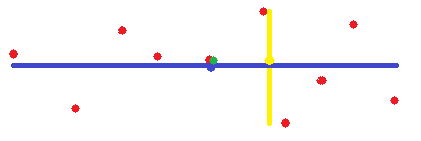
\includegraphics[width=8cm]{images/Detection/centre-object.png}
    \caption{Détermination du centre obstacle}
\end{figure}
\newline
Supposons que les points rouges correspondent à une liste de mesure que l'on a affecté à un obstacle. Le centre (vert) est alors défini en coordonnées polaire par l'angle médian (bleu) et la distance médiane (jaune).
\end{enumerate}

\subsection{Programmation en Python d'un affichage dynamique}
\tab Afin de visualiser les données extraites du LiDAR, nous avons réalisé un affichage dynamique. Cet affichage permet la visualisation des obstacles définis dans le protocole ci-dessus.
%compléter
Nous avons de plus décidé d’uniformiser les unités du code en effectuant une conversion complète des programmes en Radian.
Cela nous aura également donné l’occasion de faire un affichage ressemblant à celui d’un sonar.

\begin{figure}[htp]
    \centering
    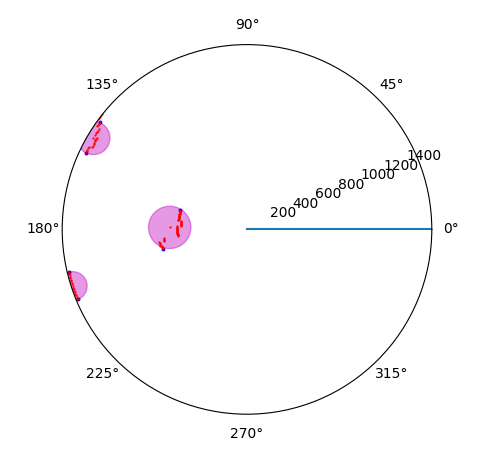
\includegraphics[width=10cm]{images/Detection/sans_piste_ni_kalman_polaire01.png}
    \caption{Affichage en coordonnées polaires.}
\end{figure}
\begin{figure}[htp]
    \centering
    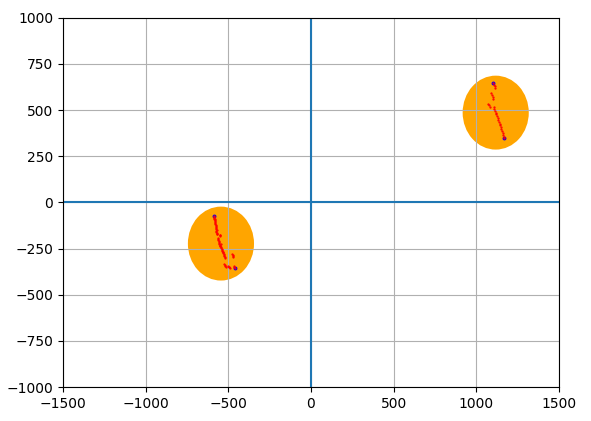
\includegraphics[width=10cm]{images/Detection/sans_piste_ni_kalman_cartesien01.png}
    \caption{Affichage en coordinnées cartesiennes.}
\end{figure}

%expliquer pourquoi on appelle ça "affichage polaire" et "affichage cartesien" ? -> Done

\newpage
\subsection{Amélioration des performances}
\tab Durant nos phases de tests, nous nous sommes rendu compte que l’élément bloquant n’était pas le traitement des données mais bel et bien l’acquisition. En effet, on s'est rendu compte que la prise de mesures sur plusieurs tours avant traitement nuisait de façon conséquente à la réactivité du système. On avait alors une rémanence des obstacles qui posait un vrai soucis.

\tab Nous avons donc décidé de paralléliser les tâches à l’aide de Threads Python pour acquérir des données en continu et de ne les récupérer que lorsque l’algorithme de traitement le demande. On a donc pu supprimer les obstacles rémanents qui nous posaient problème. Il semble en effet plus cohérent que ce soit le traitement des données qui conditionne la réactivité du système et non pas l'acquisition des données. 

\tab En définitive, le problème de l'acquisition des mesures pour la détection d'obstacle se fait de la façon la plus simple possible : on remplit progressivement une queue Python contenant les distances de chaque angle reçu, dans le sens anti-trigonométrique, chaque indice étant associé à un angle à 0.5 degré près. Le Thread principal, de traitement de données, récupère alors des éléments dans cette queue dès qu'il en a besoin. Au départ, l'idée était d'utiliser des sémaphores pour gérer l'accès à une liste, mais en utilisant des queues Python nous n'avons plus besoin de ces sémaphores explicites.

\tab Ainsi, même si on peut supposer que l'on perd en fiabilité dû au fait qu'on ne réalise plus une moyenne sur plusieurs valeurs ou bien que l'on acquiert pas nécessairement une valeur à chaque tour pour chaque angle, le gain en réactivité et la perte d'obstacles rémanents contrebalancent complètement cette perte. D'autant plus que cette perte de fiabilité, en supposant qu'elle existe, sera grandement corrigée par le traitement des obstacles, notamment avec le filtrage de Kalman.

%parler des sémaphores.  -> On s'en sert pas vraiment directement
\section{Suivi d'obstacles}

\subsection{Association d'objets}
\tab À ce stade, notre système est en mesure de nous fournir à un instant t donné / à une itération donnée, une liste d'obstacles qui ont été détectés par le LiDAR sur cette itération. Nous pourrions tout à fait nous en contenter mais l'objectif ici est d'essayer de soutirer un maximum d'informations sur nos obstacles à partir de leur position à cet instant. Concrètement, si nous sommes en mesures de savoir où cet obstacle se trouvait à l'instant précédent, nous pouvons en déduire sa vitesse instantanée. Supposons que l'on arrive à le suivre pendant plusieurs secondes, nous pouvons très bien imaginer une spéculation sur la trajectoire que va suivre l'obstacle et donc anticiper sa position sur l'itération d'après. \\
Notre problème ici est alors dans le fait d'associer les mesures entre deux instants. Comment savoir si l'obstacle X mesuré à l'instant t correspond à l'obstacle Y mesuré à l'instant $t+\Delta t$. Notre démarche a été de prendre la méthode la plus simple possible et d'essayer si cela ne suffisait pas une méthode plus complexe et plus élaborée. \cite{LIDAR2D} \cite{tutoSLAM} \cite{memoire1} \cite{MCMC-SLAM}

\subsubsection{Méthode d'association d'objet}
\tab L'association d'objet est le cœur de notre problème et de notre projet, c'est cette association qui conditionne le bon déroulement de la suite et qui conditionne la véracité de l'analyse des données du LiDAR. Notre algorithme procède donc de la façon suivante:

\begin{enumerate}
    \item Pour chaque obstacle crée à l'itération i-1 :
        \tab \begin{enumerate}
            \item On mesure sa distance par rapport à chaque obstacle créé à l'itération i
            \item On prend le minimum de cette liste de distance
            \item On vérifie que cette distance est inférieure à un seuil défini empiriquement. Ce seuil nous permet d'éviter des vitesses aberrantes si jamais on détecte un unique obstacle d'un côté à l'itération i-1 et un autre unique obstacle complètement à l'opposé à l'itération i.
            \item On considère alors que ces deux obstacles issus de l'itération i-1 et i sont les mêmes et on met alors à jour la position du dit obstacle créé à l'itération i-1.
        \end{enumerate}
    \item Si l'itération i possède plus d'obstacles que l'itération i-1, on aura des obstacles sans association, ce sont donc de nouveaux obstacles que l'on créé. 
    \item À l'inverse, si l'itération i possède moins d'obstacles que l'itération i-1, des obstacles déjà créés vont être dépourvus d'association. Cela signifie que l'obstacle n'a pas été vu à l'itération i donc que l'obstacle n'est plus présent. On détruit alors ces obstacles.
\end{enumerate}
\tab De cette façon, nous sommes en mesure d'actualiser en temps réel la position de nos obstacles.\cite{multi-target-lidar} C'est cette association qui va nous permettre de suivre les obstacles. Notre expérience sur la mise en place d'associations montre que l'utilisation de simples distances entre obstacles fonctionne plutôt bien. Il existe d'autres méthodes qui n'ont pas été développées ici mais qui sont envisageables pour améliorer le système comme l'algorithme de Kuhn-Munkres (aussi appelé algorithme hongrois) qui est un algorithme d'optimisation combinatoire et se prête bien à notre problème. Cet algorithme est notamment utilisé en surveillance pour suivre des personnes sur un flux vidéo.
%peut être parler d'un futur algo hongrois, sinon distance simple comme on l'a fait

\subsection{Détection de murs}
\tab Nous avons déterminé que les objets que nous estimons “d’intérêt” sont en réalité les murs, puisque ce sont des éléments fixes qui permettent de se repérer dans l’espace, et ainsi de les séparer des obstacles mobiles qui seront aussi à éviter. La détection de murs est aussi un élément essentiel d'algorithmes tels que SLAM. Un algorithme de \textit{RANSAC} (pour \textit{RANdom SAmple Consensus}) nous a permis de détecter ces murs afin de les rendre utilisables par d’autres algorithmes dans le cas où la plateforme robotique qui supportera notre LiDAR en aurait besoin.

% expliciter l'algorithme RANSAC en pseudo-langage

Cet algorithme est très efficace pour faire un traitement rapide d'images et obtenir rapidement les éléments linéaires d'un nuage de points, mais il a l'énorme inconvénient de ne pas être déterministe, et dans notre cas on observait qu'environ 1 fois sur 4 l'algorithme ne détectait pas certains murs, ce qui peut être risqué dans une application comme la notre. Nous avons donc décidé de ne pas l'utiliser pour le moment, et de considérer les lignes comme des obstacles comme les autres. De plus, notre objectif n'étant pas un SLAM mais seulement une localisation d'obstacles, cet algorithme n'était en aucun point essentiel.

D'autres algorithmes existent, par exemple ceux utilisant la \textit{transformée de Hough}, permettant de détecter toutes les structures linéaires dans un nuage de point. Cet algorithme, bien que plus lent, serait parfait pour notre application. Une parallélisation sur un Thread à part permettrait de continuer de traiter les données, et périodiquement récupérer les éléments linéaires des nuages de points.

% expliciter l'algorithme de Hough en pseudo-langage

%insérer image RANSAC
\subsection{Filtre de Kalman}
% détailler un peu l'aspect mathématique, ça pourrait être sympa je pense. Du moins de manière très succinte
\tab Une tâche, effectuée en parallèle avec la détection de murs, a été l'implémentation d'un Filtre de Kalman. C'est un algorithme de filtrage de données très populaire car très puissant. Il est utilisé dans toute application requérant un suivi de mesures sur une cible récupérées d'un capteur très bruité.\cite{efk}
Il comprend deux étapes qui se succèdent à chaque mise à jour des données:
\tab \begin{enumerate}
            \item \textit{Prédiction}: On utilise l'état actuel de l'objet mesuré, si il existe, pour essayer de prédire sa prochaine position réelle. On essaye aussi de prédire la matrice de covariance de l'erreur, un élément essentiel du filtre estimant entre autres la précision de l'état estimé.
            \item \textit{Mise à jour}: Après réception des nouvelles mesures, pour l'état suivant, on met à jour l'estimation de l'état de l'objet, c'est à dire son vecteur (position, vitesse), ainsi que l'estimation de sa matrice de covariance de l'erreur.
        \end{enumerate}
        
L'enchaînement de ces deux étapes permettent un suivi très peu bruité de la trajectoire des obstacles suivis. Sur l'image ci-dessous, la position mesurée est en orange, la position obtenue avec le filtre de Kalman est représentée en rouge, et les positions précédentes du centre de l'objet sont représentées en noir, ce qui constitue la \textit{piste}. En cas d'affichage de la position mesurée seulement, on verrait des trajectoires erratiques, en zig-zags de plusieurs cm de large. Ici, nous avons des courbes quasiment lisses, proches des trajectoires réelles des objets.

L'un des inconvénients au filtre de Kalman est qu'il ajoute des petits délais de réaction aux mouvements des cibles. Mais en calibrant bien le filtre nous sommes parvenus à minimiser ces délais tout en gardant des trajectoires bien fluides. Dans le cas du filtre de Kalman simple seuls sont modifiables 3 paramètres: l'écart type du processus, les écarts-types des mesures sur chaque axe, pour lesquels les valeurs empiriques optimales sont dans notre cas respectivement 15, 35mm et 35mm.
%\begin{figure}[htp]
%    \centering
%    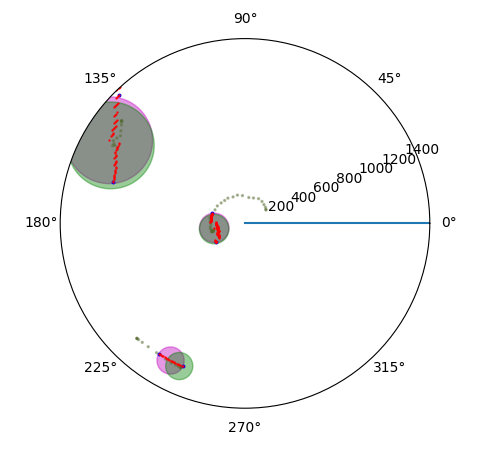
\includegraphics[width=10cm]{images/Suivi/piste01.png}
%    \caption{Piste des objets avec l'affichage polaire.}
%\end{figure}
\begin{figure}[htp]
    \centering
    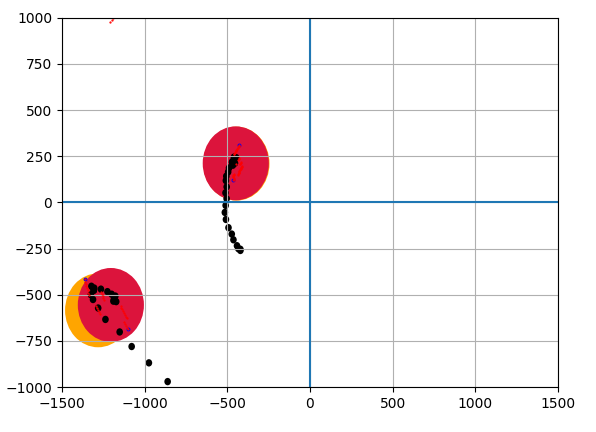
\includegraphics[width=14cm]{images/Suivi/piste02.png}
    \caption{Piste des objets avec l'affichage  cartésien.}
\end{figure}
\section{Intégration du LiDAR sur une plateforme robotique}
\subsection{Integration mécanique}
\tab Il a fallu là aussi réfléchir à la meilleure option compte tenu de notre système. Le robot sur lequel nous posons le LiDAR participe à la Coupe de France de Robotique. Le règlement de la coupe impose à tout participant d'avoir un robot dont la hauteur n'excède pas 35cm. Cependant, ils doivent tous avoir un support de balise de 8cm de haut à une hauteur de 35cm jusqu'à 43cm. Ce support balise doit être opaque et suffisamment gros (cylindre de 70 à 100m de diamètre positionné au centre du robot). Comme nous n'avons aucune assurance sur la taille d'un robot adverse et que c'est l'élément principal si ce n'est le seul que nous voulons détecter, nous ne pouvons essayer de détecter à la hauteur que nous voulons. Nous avons donc fait le choix de mettre le LiDAR à l'intérieur du support balise. En effet, comme nous avons le droit à un trou jusqu'à 2cm de hauteur sur le support de balise, nous pouvons l'intégrer à l'intérieur dans l'espoir de détecter le support balise de l'adversaire. Comme nous sommes certains que tous les robots posséderont un support balise, nous sommes confiants sur la possibilité de détecter l'adversaire.

\begin{figure}[htp]
    \centering
    \includegraphics[width=6cm]{images/Integration/integration_robot.jpg}
    \caption{Début du montage sur le robot.}
\end{figure}

\begin{figure}[htp]
    \centering
    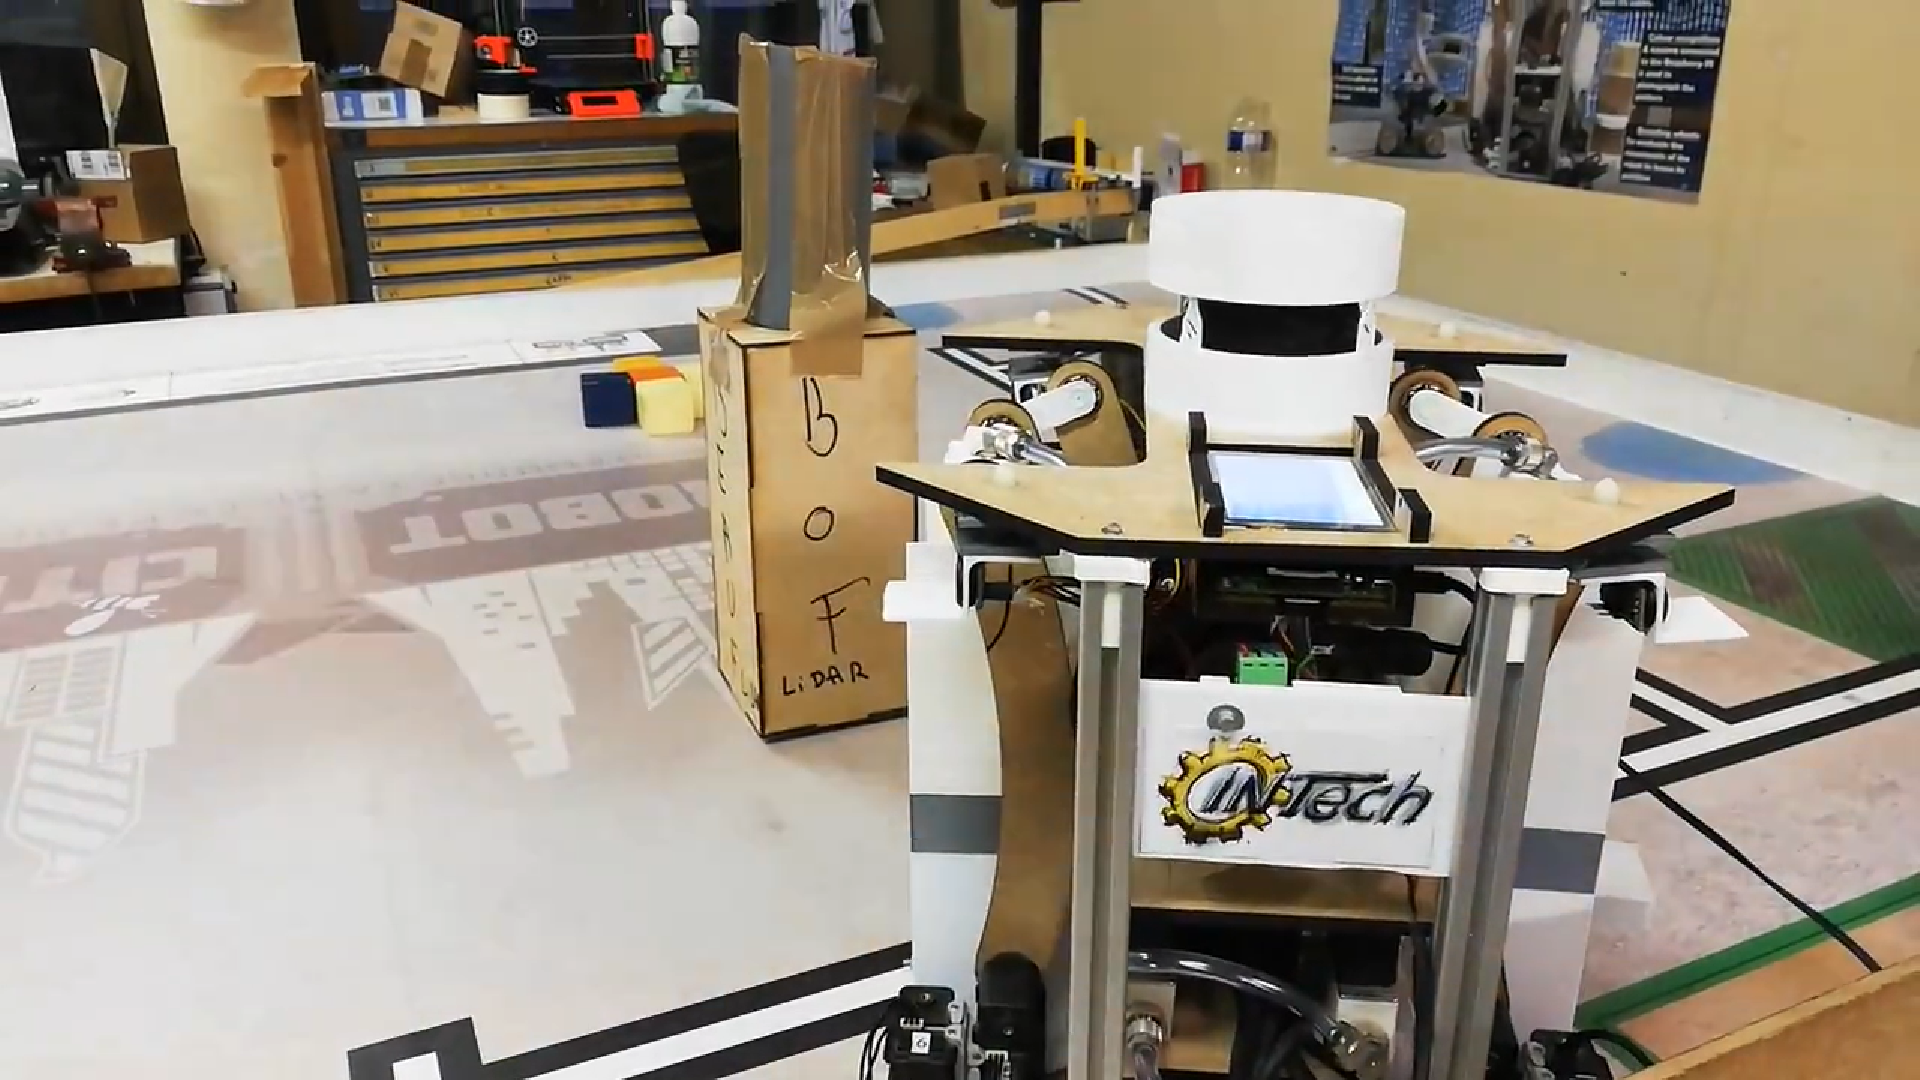
\includegraphics[width=6cm]{images/Integration/robot_intech.png}
    \caption{LiDAR en action sur le robot INTech.}
\end{figure}

\subsection{Interfaçage avec le pathfinding}
% probleme RPI => CODE C

\tab L'objectif était de pouvoir envoyer la position des obstacles détectés à un code en Java qui contenait la gestion complète de la stratégie du robot du club de robotique INTech. Ce code implémentait donc notamment un \textit{pathfinding} qui avait vocation à traiter les informations fournies par notre code associé au LiDAR.  

Après discussion, la solution adoptée a été la suivante:
\begin{enumerate}
    \item lancer notre code Python à partir du code Java
    \item créer une \textit{socket} afin d'envoyer le centre de la position de chaque obstacle au code Java
    \item le \textit{pathfinding} peut alors utiliser ces informations pour calculer un nouveau chemin et éviter un potentiel obstacle
\end{enumerate}
\tab L'interfaçage avec le \textit{pathfinding} a été réalisé avec succès, mais a soulevé un nouveau problème : sur le Raspberry Pi la capacité de la série python pour lire les informations envoyées par le LiDAR est trop faible, conduisant à une latence croissante au fur et à mesure que l'on effectue des mesures. Ce problème n'apparaissait pas lors de nos tests sur ordinateur, et il s'est avéré que d'autres personnes ont eu le même problème sur Raspberry Pi, y compris en utilisant des librairies C. Le problème semble donc venir de l'implémentation série sur ARM. Une solution trouvée a été de réécrire un code C à la main, permettant de lire très rapidement depuis le LiDAR, sans utiliser des librairies qui sur Raspberry Pi semblent lire trop lentement pour nos besoins.
%On a pas encore testé sur Raspi le code C... Faudrait chopper Julian demain si vous pouvez et le harceler pour filer son code

\subsection{Résultat final}

\tab Ici on peut voir le robot INTech en pleine esquive pour atteindre les cubes visibles dans le fond de l'image. Ci-contre la vidéo:  \href{https://drive.google.com/open?id=1gUHL_6yfKHhAX55Kx0Wif0i2wZ0wc-EG}{Lien de la vidéo.}\footnote{https://drive.google.com/open?id=1gUHL\_6yfKHhAX55Kx0Wif0i2wZ0wc-EG}

On peut également observer le robot et son LiDAR en plein match lors de la Coupe d'Île de France 2018 :
\href{https://drive.google.com/open?id=1vG5ts-w3lH8zYN6OM3irqqE8x8yshUWw}{Lien de la vidéo.}\footnote{https://drive.google.com/open?id=1vG5ts-w3lH8zYN6OM3irqqE8x8yshUWw}

\section*{Conclusion}
\addcontentsline{toc}{section}{Conclusion}
\markboth{Conclusion}{Conclusion}
\tab Ce projet, que nous avons porté pendant plusieurs mois, nous a permis de partir d'un LiDAR ,dont la documentation est claire mais peu complète, pour aller jusqu'à un code complet permettant de mettre à profit les capacité de ce capteur. Finalement, nous avons dû sortir de notre code en Python non seulement pour nous plonger de longues heures dans la documentation, mais également pour étudier le fonctionnement de la série sur nos ordinateurs classiques et sur des architectures ARM, et tenter d'améliorer les performances de notre implémentation.

\tab L'intégration au robot du club INTech a été l'élément clé qui nous a permis de réaliser le travail accompli et de le voir à l'oeuvre. 
%écrivez d'autres trucs si vous êtes inspirés

%et ajouter annexes

\appendix
\bibliographystyle{authoryear-fr}
\bibliography{cassiopee}
\nocite{*}
%%%%%%%%%%%%%%%%
%%% Abstract %%% d'après la docu il est sensé y avoir un fichier isae-report-template.tex, il est plus là?

\end{document}